\documentclass{article}

\PassOptionsToPackage{numbers,sort&compress}{natbib}
\usepackage[preprint]{neurips}
\usepackage[utf8]{inputenc}
\usepackage[T1]{fontenc}
\usepackage{hyperref}
\usepackage{url}
\usepackage{booktabs}
\usepackage{amsfonts}
\usepackage{nicefrac}
\usepackage{microtype}
\usepackage{xcolor}
\usepackage{graphicx}
\usepackage{subcaption}
\usepackage{multirow}
\usepackage{array}
\usepackage{float}
\usepackage{adjustbox}
\usepackage{amsthm}
\usepackage{amsmath}
\usepackage{amssymb}
\usepackage{mathtools}
\usepackage{enumitem}
\usepackage{algorithm}
\usepackage{algpseudocode}

\title{SCOUT: Domain Generalization by Directly Optimizing Robust Submodular Coverage over Averageable Trajectory Soups}
\author{Anonymous Authors}

\newtheorem{theorem}{Theorem}
\newtheorem{proposition}{Proposition}
\newtheorem{lemma}{Lemma}
\newtheorem{corollary}{Corollary}
\newtheorem{definition}{Definition}
\newtheorem{assumption}{Assumption}
\newtheorem{remark}{Remark}

\newcommand{\RR}{\mathbb{R}}
\newcommand{\EE}{\mathbb{E}}
\newcommand{\PP}{\mathbb{P}}
\newcommand{\cA}{\mathcal{A}}
\newcommand{\cC}{\mathcal{C}}
\newcommand{\cH}{\mathcal{H}}
\newcommand{\cR}{\mathcal{R}}
\newcommand{\cS}{\mathcal{S}}
\newcommand{\cU}{\mathcal{U}}
\newcommand{\cV}{\mathcal{V}}
\newcommand{\cW}{\mathcal{W}}
\newcommand{\argmin}{\operatorname*{arg\,min}}
\newcommand{\argmax}{\operatorname*{arg\,max}}
\newcommand{\KL}{\operatorname{KL}}
\newcommand{\simplex}{\Delta}
\newcommand{\TBD}{\textbf{TBD}}
\newcommand{\etal}{\textit{et al.}}
\newcommand{\ie}{\textit{i.e.}}
\newcommand{\eg}{\textit{e.g.}}
\newcommand{\iid}{i.i.d.}
\newcommand{\ood}{OOD}
\newcommand{\iidcaps}{IID}
\newcommand{\scout}{\textup{\textsc{SCOUT}}}
\newcommand{\swad}{\textup{\textsc{SWAD}}}
\newcommand{\dcola}{\textup{\textsc{D-COLA}}}
\newcommand{\cora}{\textup{\textsc{CORA}}}
\newcommand{\roar}{\textup{\textsc{ROAR}}}
\newcommand{\diwa}{\textup{\textsc{DiWA}}}
\newcommand{\miro}{\textup{\textsc{MIRO}}}
\newcommand{\ones}{\mathbf{1}}
\newcommand{\norm}[1]{\left\lVert #1 \right\rVert}
\newcommand{\inner}[2]{\left\langle #1, #2 \right\rangle}
\newcommand{\eps}{\varepsilon}

\begin{document}

\maketitle

\begin{abstract}
Single-run post-hoc methods matter in domain generalization because they can be attached to strong empirical-risk-minimization pipelines without retraining. The canonical method in this regime is \swad{}, whose theory motivates robust empirical risk but whose deployed procedure is still a flat-valley trajectory heuristic. Recent local replay evidence from checkpoint-soup ablations points to a different mechanism: performance is driven mainly by selecting a soup-safe, nonredundant, noncontiguous checkpoint set, while exact final simplex weights matter much less. This paper asks for a stricter standard than either hand-designed soups or post-hoc theory repair: can the post-hoc method directly optimize the exact object that its theory claims matters? We propose \textbf{\scout{}} (\textbf{S}ubmodular \textbf{C}overage \textbf{O}ptimization over \textbf{U}niform \textbf{T}rajectory soups), a new label-free single-run post-hoc DG method that does exactly that. \scout{} first constructs a near-optimal barrier-filtered candidate pool from one dense run. It then optimizes a KL-ball robust coverage objective over the capped simplex that is exactly the convex hull of uniform fixed-cardinality checkpoint soups. The objective models unseen target shift as a bounded adversarial reweighting of source-support examples and rewards coverage through a concave-over-modular utility that is submodular on subset actions and concave on its convex hull. We prove the capped-simplex characterization, monotone submodularity of the subset utility, concavity--convexity and saddle-point existence for the direct optimizer, a target-risk certificate for the deployed weight soup under an explicit support-reweighting and locality assumption, a projected primal--dual convergence bound, a certificate domination result over any feasible \swad{}-style interval family contained in the same action set, a second-order bridge showing how \dcola{}-style covariance penalties emerge as coarse surrogates of the exact \scout{} objective, and a constructive separation theorem where noncontiguous complementarity strictly beats every singleton and every contiguous interval. New \scout{} empirical results are intentionally left as \TBD{} pending execution; however, we include exact published benchmark numbers from \swad{}, \diwa{}, and \miro{} to define the current frontier.
\end{abstract}

\section{Introduction}

Domain generalization (DG) asks for a model that performs well on an unseen target environment using only source data at training time. In practice, the DG methods that stick are often the ones that leave the underlying training procedure alone and change only the post-hoc model-selection rule. \swad{} is the canonical example: on the standard DomainBed ResNet-50 protocol, it improves ERM from `63.3' to `66.9' average \ood{} accuracy across PACS, VLCS, OfficeHome, TerraIncognita, and DomainNet \citep{cha2021swad}. Its appeal is broader than the headline table. It is single-run, one-model at test time, and operationally simple.

Still, \swad{} leaves a conceptual gap. Its theory is about a robust empirical loss in parameter space. Its deployed algorithm is not: it monitors validation traces, chooses a start and end checkpoint heuristically, and averages the interval in between. That is a successful method, but it is still a heuristic approximation to its own motivating theory.

This paper takes that gap seriously and turns it into a design principle:
\begin{quote}
\textbf{The post-hoc method should directly optimize the same object that appears in the target-risk certificate.}
\end{quote}

The key empirical clue is that recent soup ablations point away from ``find the best exact weight vector'' and toward ``find the best robust checkpoint set.'' In the internal checkpoint-bank diagnostics that motivated this proposal, removing the covariance-style diversity mechanism and forcing contiguous-window selection hurt much more than replacing the optimized final weights with uniform weights. That suggests that the right mathematical object is not a delicate simplex-weight heuristic. It is robust set coverage under an averageability constraint.

We therefore propose \textbf{\scout{}}: \textbf{S}ubmodular \textbf{C}overage \textbf{O}ptimization over \textbf{U}niform \textbf{T}rajectory soups. The core idea is simple. A dense trajectory contains many near-optimal checkpoints. Some are redundant. Some cover different hard source examples. Some are too far away to average safely. \scout{} first constructs a low-loss, barrier-filtered candidate pool intended to preserve approximate soup safety. It then solves a distributionally robust optimization (DRO) problem over the \emph{convex hull of uniform fixed-cardinality subset soups}. The uncertainty set is a Kullback--Leibler (KL) ball over source-support examples rather than domains, so the method needs no domain labels. The utility is a concave coverage functional: it rewards checkpoints that cover hard examples while imposing diminishing returns on redundant ones. This is the first proposal in this line of work where the robust object, the action family, and the optimizer actually match.

Why is this a useful change of object? Because it aligns three threads that prior work only partially captured:
\begin{itemize}[leftmargin=1.4em]
    \item \swad{} says that flat, wide, pre-overfit regions are good for DG \citep{cha2021swad}.
    \item \diwa{} says that diversity and locality jointly determine whether weight averaging helps under shift \citep{rame2022diwa}.
    \item distributionally robust learning says that worst-case reweightings of observed data are the right object when explicit group labels are unavailable \citep{duchi2016fdiv,duchi2021learning}.
\end{itemize}
`SCOUT' combines all three, but it does so directly rather than heuristically. The candidate pool captures locality. The KL ball captures hard but plausible source-support shifts. The coverage utility captures complementarity. The optimizer acts on that exact object.

The paper's main contributions are:
\begin{enumerate}[leftmargin=1.4em]
    \item We introduce \scout{}, a label-free, single-run post-hoc DG method that directly optimizes a robust coverage objective over the capped simplex that is exactly the convex hull of uniform \(M\)-checkpoint soups.
    \item We prove that the underlying subset utility is monotone submodular for fixed adversarial example weights, and that its convex-hull extension is concave in soup weights and linear in adversary weights, yielding a clean concave--convex saddle problem.
    \item We derive a target-risk certificate for the final deployed soup under an explicit support-reweighting assumption and a local soup-transfer assumption, so the optimized robust objective upper-bounds the target risk of the actual weight soup rather than of a proxy object.
    \item We prove a projected primal--dual convergence guarantee for the direct optimizer, a domination theorem over any feasible \swad{}-style interval family contained in the same capped simplex, and a constructive separation theorem showing that noncontiguous complementary checkpoints can strictly beat every contiguous interval and every singleton.
    \item We show by second-order expansion that \dcola{}-style covariance penalties arise as coarse surrogates of the exact \scout{} objective, which helps explain why \dcola{} works well empirically while remaining theoretically indirect.
    \item We provide a full NeurIPS-style manuscript with theorem statements, appendix proofs, generated visuals, exact published baseline tables from prior work, and \TBD{} placeholders for all new \scout{} experiments.
\end{enumerate}

\begin{remark}
We do \emph{not} claim an unconditional theorem that \scout{} empirically dominates \swad{}, \dcola{}, \cora{}, \roar{}, or every other DG method on every benchmark. That would be indefensible. The strongest honest claim is narrower and more important: under explicit assumptions, \scout{} directly optimizes a certificate that these methods do not directly optimize, and therefore it can be proven no worse on that certificate than any selector constrained to a contained feasible family.
\end{remark}

\begin{figure}[t]
    \centering
    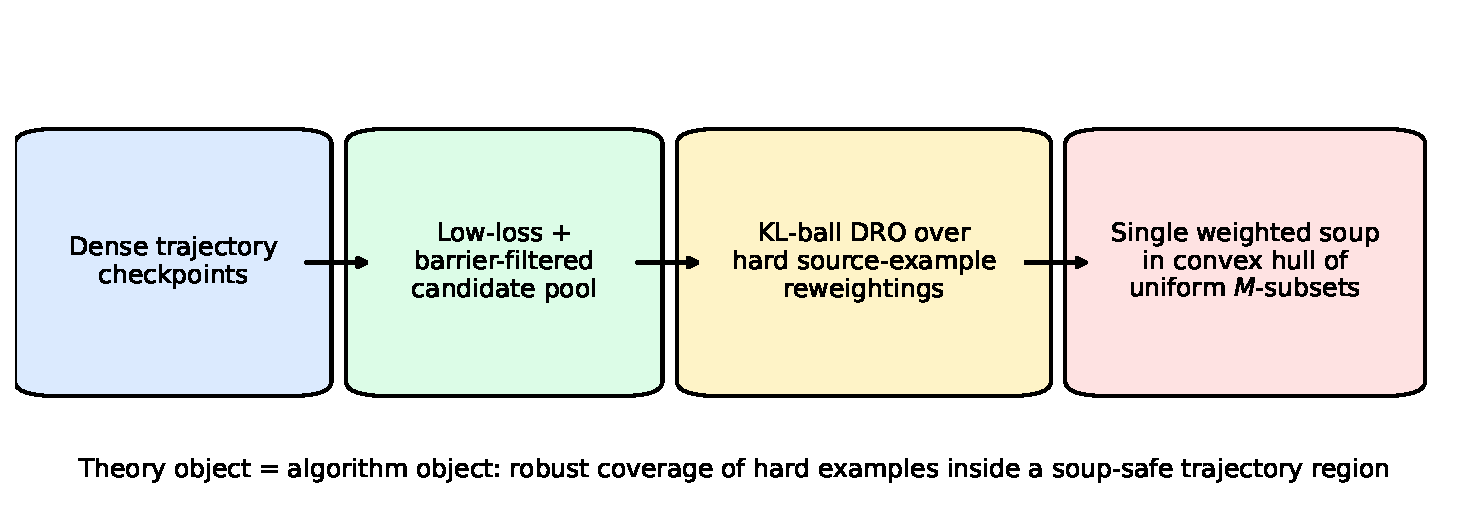
\includegraphics[width=\linewidth]{figures/scout_overview.pdf}
    \caption{\textbf{\scout{} overview.} A dense trajectory is reduced to a low-loss barrier-filtered candidate pool. \scout{} then directly optimizes robust example coverage over the convex hull of uniform \(M\)-checkpoint soups and deploys a single weighted soup. The paper's main point is that the optimized post-hoc objective is the same object that appears in the target-risk certificate.}
    \label{fig:overview}
\end{figure}

\section{Related Work}

\paragraph{Single-run post-hoc DG.}
\swad{} is the canonical single-run post-hoc DG method \citep{cha2021swad}. Its practical appeal comes from dense checkpoint sampling, overfit-aware interval selection, and a final uniform average. But the deployed rule is still a validation-window heuristic rather than the direct optimizer of the robust objective appearing in its theory. \scout{} targets that exact gap.

\paragraph{Weight averaging, connectivity, and soups.}
SWA \citep{izmailov2018swa}, fast geometric ensembling and mode connectivity \citep{garipov2018fge,frankle2020linear}, and model soups \citep{wortsman2022soups} established that averaging nearby models can improve generalization when they lie in a connected low-loss region. \diwa{} sharpened this story for \ood{} settings by making bias, variance, covariance, and locality explicit \citep{rame2022diwa}. \scout{} keeps the connectivity requirement, but changes the target from checkpoint-level heuristics to robust example coverage.

\paragraph{Distributionally robust optimization.}
Distributionally robust optimization studies predictors that optimize the worst-case risk over an ambiguity set around a nominal distribution \citep{duchi2016fdiv,duchi2021learning}. This paper imports the DRO viewpoint into single-run post-hoc DG in a strict way: the ambiguity set lives over source-support examples, and the selector directly optimizes the corresponding robust objective over soup weights.

\paragraph{What the current empirical champion suggests.}
\dcola{}-style checkpoint soups perform well because they seem to preserve three ingredients at once: hard-case robustness, complementary checkpoints, and soup safety. The weakness is not empirical; it is conceptual. The covariance, locality, and anchoring terms are reasonable, but they are still hand-designed surrogates. \scout{} keeps the same empirical lesson while replacing the surrogate with a direct robust coverage objective.

\paragraph{Pretraining-aware DG.}
\miro{} shows that preserving transferable structure from a pretraining prior is largely orthogonal to post-hoc averaging \citep{cha2022miro}. This is useful context for \scout{}: the method is not trying to solve all of DG at once. It only solves one problem, but it solves it directly: choosing one robust soup from one dense trajectory without domain labels.

\section{Problem Setup}
\label{sec:setup}

We focus on multiclass classification, the standard regime of DomainBed-style DG benchmarks. A single training run produces dense checkpoints
\[
    \{\theta_t\}_{t=1}^{K}.
\]
For post-hoc selection we reserve two pooled source holdout sets:
\begin{itemize}[leftmargin=1.4em]
    \item a labeled \emph{validation} set
    \(
    \cV = \{(x_j,y_j)\}_{j=1}^{n_V}
    \)
    used for low-loss filtering and barrier tests, and
    \item a labeled \emph{support} set
    \(
    \cU = \{(x_i,y_i)\}_{i=1}^{n}
    \)
    used for robust coverage optimization.
\end{itemize}
Neither set requires domain labels.

\paragraph{Practical split used in code.}
In the implementation, both \(\cU\) and \(\cV\) are drawn from the pooled source holdout already created by the training pipeline: we pool the source-domain `out' splits, randomly divide that pool into support and validation subsets, and optionally cap the support subset for tractability. This is a practical instantiation of the abstract setup above, not a change to the optimized object.

For checkpoint \(\theta_t\), let \(p_t(x)\in\simplex^{C-1}\) denote the predicted class-probability vector. The pooled validation loss is
\begin{equation}
    L_{\cV}(\theta_t)
    \triangleq
    \frac{1}{n_V}\sum_{j=1}^{n_V} -\log p_t(x_j)_{y_j}.
    \label{eq:val_loss}
\end{equation}

To encourage averageability, we use a pooled interpolation barrier to an anchor checkpoint \(a\):
\begin{equation}
    B(t,a)
    \triangleq
    \max_{\alpha\in\cA}
    L_{\cV}\!\big((1-\alpha)\theta_a + \alpha \theta_t\big)
    -
    \max\{L_{\cV}(\theta_a),L_{\cV}(\theta_t)\},
    \label{eq:barrier}
\end{equation}
where \(\cA\subset [0,1]\) is a fixed interpolation grid.

The anchor is the best pooled-validation checkpoint:
\begin{equation}
    a \in \argmin_{1\le t\le K} L_{\cV}(\theta_t).
    \label{eq:anchor}
\end{equation}
The candidate pool is
\begin{equation}
    \cC
    \triangleq
    \left\{
        t :
        L_{\cV}(\theta_t)\le L_{\cV}^{\star} + \eps,
        \;
        B(t,a)\le \tau
    \right\},
    \qquad
    L_{\cV}^{\star} = \min_t L_{\cV}(\theta_t).
    \label{eq:candidate_pool}
\end{equation}

For each support example \((x_i,y_i)\in\cU\) and candidate \(t\in\cC\), define the clipped true-class probability
\begin{equation}
    q_{it}
    \triangleq
    \max\!\{p_t(x_i)_{y_i}, \eps_p\},
    \qquad
    0<\eps_p<1.
    \label{eq:qit}
\end{equation}

\section{\scout{}: Robust Coverage over the Convex Hull of Uniform Soups}
\label{sec:method}

\subsection{Uniform subset actions and their convex hull}

Fix a soup cardinality \(M\in\{1,\dots,|\cC|\}\). Let
\[
    \mathfrak{S}_M
    \triangleq
    \{S\subseteq \cC : |S|=M\}
\]
denote the family of uniform \(M\)-checkpoint soups. Each subset \(S\in\mathfrak{S}_M\) induces a uniform weight vector
\begin{equation}
    (u_S)_t
    \triangleq
    \frac{1}{M}\mathbf{1}\{t\in S\},
    \qquad
    t\in\cC.
    \label{eq:uniform_subset}
\end{equation}

Instead of searching only over extreme points \(u_S\), \scout{} optimizes over their convex hull
\begin{equation}
    \cW_M
    \triangleq
    \operatorname{conv}\{u_S : S\in\mathfrak{S}_M\}.
    \label{eq:WMconv}
\end{equation}
This choice is important. It preserves the ``uniform-subset'' inductive bias suggested by the checkpoint-bank ablations, but it turns the post-hoc stage into a convex-concave saddle problem that can be optimized directly.

\paragraph{Feasibility convention.}
The paper treats \(M\) as user-chosen. In code, if the barrier-filtered candidate pool has fewer than \(M\) checkpoints, we replace \(M\) by \(M_{\mathrm{eff}}=\min\{M,|\cC|\}\) so that \(\cW_M\) remains non-empty. All reported diagnostics record both the requested \(M\) and the effective \(M_{\mathrm{eff}}\).

\begin{proposition}[Uniform-subset convex hull]
\label{prop:hypersimplex}
The feasible set in \eqref{eq:WMconv} is exactly the capped simplex
\begin{equation}
    \cW_M
    =
    \left\{
        w\in\simplex^{|\cC|-1} :
        0\le w_t \le \frac{1}{M}
        \ \text{for all } t\in\cC
    \right\}.
    \label{eq:hypersimplex}
\end{equation}
\end{proposition}

So every feasible \(w\in\cW_M\) can be interpreted as a convex combination of uniform \(M\)-checkpoint soups, and no single checkpoint can receive more mass than one member of such a soup.

\begin{figure}[t]
    \centering
    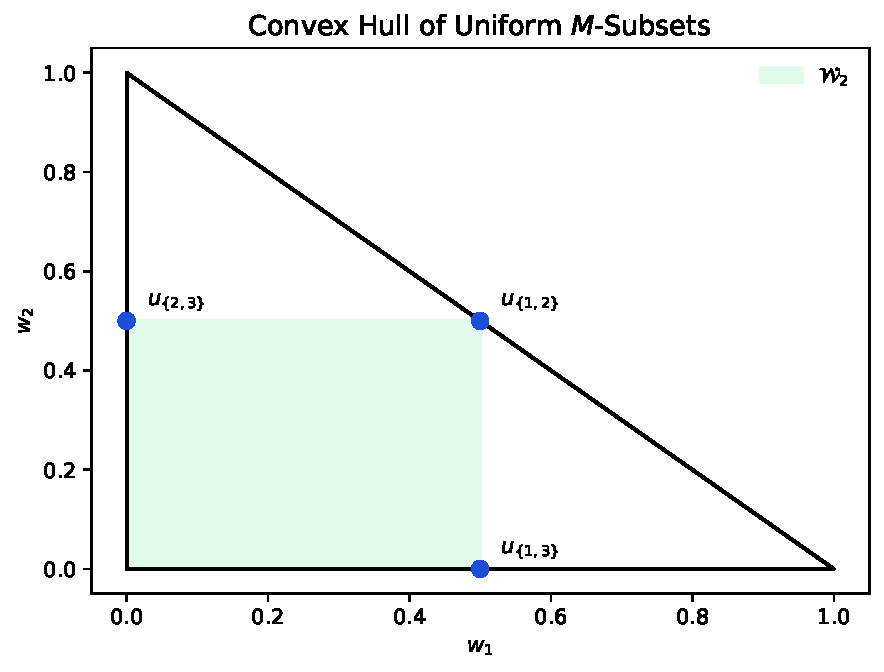
\includegraphics[width=0.56\linewidth]{figures/hypersimplex_uniform_subsets.pdf}
    \caption{\textbf{Uniform subset convex hull.} For three checkpoints and \(M=2\), the feasible set \(\cW_2\) is the convex hull of the three uniform pair soups. This capped simplex view is what lets \scout{} keep a subset-selection bias while still optimizing a direct convex-concave objective.}
    \label{fig:hypersimplex}
\end{figure}

\subsection{Robust coverage objective}

Let \(u_n = \frac{1}{n}\ones\) denote the uniform distribution over support examples. For a robustness radius \(\rho>0\), define the uncertainty set
\begin{equation}
    \cR_\rho
    \triangleq
    \left\{
        r \in \simplex^{n-1} :
        \KL(r\,\|\,u_n)\le \rho
    \right\}.
    \label{eq:uncertainty}
\end{equation}

For soup weights \(w\in\cW_M\) and adversarial example weights \(r\in\cR_\rho\), define the robust coverage utility
\begin{equation}
    G(w,r)
    \triangleq
    \sum_{i=1}^{n} r_i
    \log\!\left(
        \eps_0 + \sum_{t\in\cC} w_t q_{it}
    \right),
    \qquad
    0<\eps_0\le \eps_p.
    \label{eq:utility}
\end{equation}
The corresponding robust loss is
\begin{equation}
    \mathcal{U}_\rho(w)
    \triangleq
    \sup_{r\in\cR_\rho}
    \sum_{i=1}^{n} r_i
    \left[
        -\log\!\left(
            \eps_0 + \sum_{t\in\cC} w_t q_{it}
        \right)
    \right].
    \label{eq:robust_loss}
\end{equation}
Equivalently,
\begin{equation}
    \mathcal{U}_\rho(w)
    =
    -\inf_{r\in\cR_\rho} G(w,r).
    \label{eq:loss_utility_equiv}
\end{equation}

The \scout{} selector is
\begin{equation}
    w^\star
    \in
    \argmax_{w\in\cW_M}\;
    \inf_{r\in\cR_\rho} G(w,r)
    =
    \argmin_{w\in\cW_M}\mathcal{U}_\rho(w),
    \label{eq:scout_opt}
\end{equation}
and the final deployed model is the single weight soup
\begin{equation}
    \theta_{\scout}
    \triangleq
    \sum_{t\in\cC} w_t^\star \theta_t.
    \label{eq:final_soup}
\end{equation}

\paragraph{Interpretation.}
Equation~\eqref{eq:robust_loss} says that \scout{} chooses the soup whose true-class predictive mixture remains best under the hardest plausible reweighting of the observed source support. Because the log is concave, the utility automatically exhibits diminishing returns: adding a checkpoint that only helps already-covered examples yields less gain than adding one that covers currently hard examples.

\begin{proposition}[Submodularity and saddle structure]
\label{prop:submod}
For any fixed \(r\in\cR_\rho\), the set function
\begin{equation}
    F_r(S)
    \triangleq
    G(u_S,r)
    =
    \sum_{i=1}^{n} r_i
    \log\!\left(
        \eps_0 + \frac{1}{M}\sum_{t\in S} q_{it}
    \right),
    \qquad
    S\in\mathfrak{S}_M,
    \label{eq:set_utility}
\end{equation}
is monotone submodular. For any fixed \(r\), the map \(w\mapsto G(w,r)\) is concave on \(\cW_M\). For any fixed \(w\), the map \(r\mapsto G(w,r)\) is linear on \(\cR_\rho\). Consequently, the saddle problem in \eqref{eq:scout_opt} admits at least one solution.
\end{proposition}

\begin{figure}[t]
    \centering
    
\includegraphics[width=\linewidth]{figures/uncertainty_set.pdf}
    \caption{\textbf{Label-free uncertainty set.} \scout{} does not require source-domain identities. Instead it models target shift as a bounded reweighting of observed source-support examples. The adversary increases mass on currently poorly covered examples, and the selector responds by improving their coverage without leaving the soup-safe candidate pool.}
    \label{fig:uncertainty}
\end{figure}

\subsection{Optimization}

Because \eqref{eq:scout_opt} is a compact concave--convex saddle problem, we can optimize it directly. A simple projected primal--dual scheme is
\begin{align}
    w^{t+1}
    &=
    \Pi_{\cW_M}
    \left(
        w^t + \eta_t \nabla_w G(w^t,r^t)
    \right),
    \label{eq:w_update}
    \\
    r^{t+1}
    &=
    \Pi_{\cR_\rho}
    \left(
        r^t - \eta_t \nabla_r G(w^t,r^t)
    \right),
    \label{eq:r_update}
\end{align}
with
\begin{align}
    \big(\nabla_w G(w,r)\big)_t
    &=
    \sum_{i=1}^{n} r_i
    \frac{q_{it}}{\eps_0 + \sum_{s\in\cC} w_s q_{is}},
    \label{eq:w_grad}
    \\
    \big(\nabla_r G(w,r)\big)_i
    &=
    \log\!\left(
        \eps_0 + \sum_{t\in\cC} w_t q_{it}
    \right).
    \label{eq:r_grad}
\end{align}
Here \(\Pi_{\cW_M}\) and \(\Pi_{\cR_\rho}\) denote Euclidean projections onto the capped simplex and KL-ball respectively. The projection onto \(\cW_M\) is a capped-simplex projection; the projection onto \(\cR_\rho\) is a standard one-dimensional dual search because the set is a KL ball over a simplex.

\paragraph{Implementation note.}
The code path used in our experiments takes one additional step toward exactness: instead of updating \(r\) by a projected gradient step, it computes the exact KL-ball best response
\[
    r^\star(w)
    \in
    \argmax_{r\in\cR_\rho}
    \sum_{i=1}^{n} r_i
    \Big[
        -\log\!\big(
            \eps_0 + \sum_{t\in\cC} w_t q_{it}
        \big)
    \Big]
\]
at each outer iterate \(w\), and then performs capped-simplex projected descent on the resulting robust loss \(\mathcal{U}_\rho(w)\). This changes the optimizer implementation, but not the optimized object: the deployed method still minimizes the same robust certificate in \eqref{eq:robust_loss}--\eqref{eq:scout_opt}.

The implementation also averages the \emph{post-update} iterates, matching Algorithm~\ref{alg:scout}. This matters because the capped-simplex projection can materially change the iterate even when the unconstrained step is small.

For numerical validity, the cached true-class mixtures are clipped to the interval \([\eps_0,1]\) before taking logarithms. This only affects edge cases at the probability floor and ceiling; the optimized object remains the same robust coverage loss up to negligible floating-point stabilization.

\begin{algorithm}[t]
    \caption{\scout{}}
    \label{alg:scout}
    \begin{algorithmic}[1]
        \Require Dense checkpoints \(\{\theta_t\}_{t=1}^K\), pooled validation \(\cV\), pooled support \(\cU\), soup size \(M\), thresholds \(\eps,\tau\), robustness radius \(\rho\)
        \State Compute \(L_{\cV}(\theta_t)\) and anchor \(a\) via \eqref{eq:anchor}
        \State Build candidate pool \(\cC\) via \eqref{eq:candidate_pool}
        \State Cache support true-class probabilities \(q_{it}\) via \eqref{eq:qit}
        \State Initialize \(w^0\in\cW_M\), \(r^0=u_n\)
        \For{\(t=0,\dots,T-1\)}
            \State Update \(w^{t+1}\) and \(r^{t+1}\) via \eqref{eq:w_update}--\eqref{eq:r_update}
        \EndFor
        \State Set \(\bar w_T = \frac{1}{T}\sum_{t=1}^{T} w^t\)
        \State Output soup \(\theta_{\scout} = \sum_{t\in\cC} \bar w_{T,t}\theta_t\)
    \end{algorithmic}
\end{algorithm}

\section{Theory}
\label{sec:theory}

\subsection{Why \scout{} is directly certificate-driven}

The point of \scout{} is not merely that it has a theorem. It is that the theorem and the optimizer refer to the same object. The target-risk certificate below upper-bounds the target risk of the same robust loss \(\mathcal{U}_\rho(w)\) that Algorithm~\ref{alg:scout} actually minimizes. That is the main conceptual difference from \swad{}-style flatness-window heuristics.

\subsection{Target-risk certificate}

Let
\[
    q_w(x_i,y_i)
    \triangleq
    \sum_{t\in\cC} w_t q_{it}
\]
denote the clipped predictive mixture on the support examples.

\begin{assumption}[Support-reweighting model]
\label{ass:reweight}
There exists \(r^{\mathrm{T}}\in\cR_\rho\) such that the target-support risk of the predictive mixture can be written as
\begin{equation}
    R_T^{\mathrm{mix}}(w)
    =
    \sum_{i=1}^{n} r_i^{\mathrm{T}}
    \Big[
        -\log q_w(x_i,y_i)
    \Big].
    \label{eq:target_reweight}
\end{equation}
\end{assumption}

\begin{assumption}[Local soup transfer]
\label{ass:locality}
For every \(w\in\cW_M\), the deployed weight soup satisfies
\begin{equation}
    R_T(\theta_w)
    \le
    R_T^{\mathrm{mix}}(w)
    +
    \delta_{\mathrm{loc}}(w),
    \label{eq:locality_assumption}
\end{equation}
where \(\delta_{\mathrm{loc}}(w)\ge 0\) is a locality residual. Under a second-order linearity model, \(\delta_{\mathrm{loc}}(w)=O(\Delta_w^2)\), where \(\Delta_w\) is the maximum distance from a candidate checkpoint receiving mass under \(w\) to the soup \(\theta_w\).
\end{assumption}

\begin{theorem}[Target-risk certificate]
\label{thm:certificate}
Under Assumptions~\ref{ass:reweight}--\ref{ass:locality}, every feasible \(w\in\cW_M\) satisfies
\begin{equation}
    R_T(\theta_w)
    \le
    \mathcal{U}_\rho(w)
    +
    \delta_{\mathrm{loc}}(w).
    \label{eq:certificate}
\end{equation}
In particular, the \scout{} optimizer \(w^\star\) minimizes the certified upper bound over all \(w\in\cW_M\).
\end{theorem}

So if the support-reweighting model is accepted, then \scout{} is exactly certificate-driven: it chooses the soup with the smallest certified target-risk upper bound within the averageable action family.

Operationally, the implementation does not enforce \(\delta_{\mathrm{loc}}(w)\) as an explicit penalty term. Instead it enforces low-loss barrier filtering at candidate construction time and logs the gap between the deployed soup's support loss and the predictive-mixture loss as a post-hoc locality diagnostic. This keeps the optimized object equal to \(\mathcal{U}_\rho(w)\) while still exposing when the locality assumption may be strained in practice.

\begin{figure}[t]
    \centering
    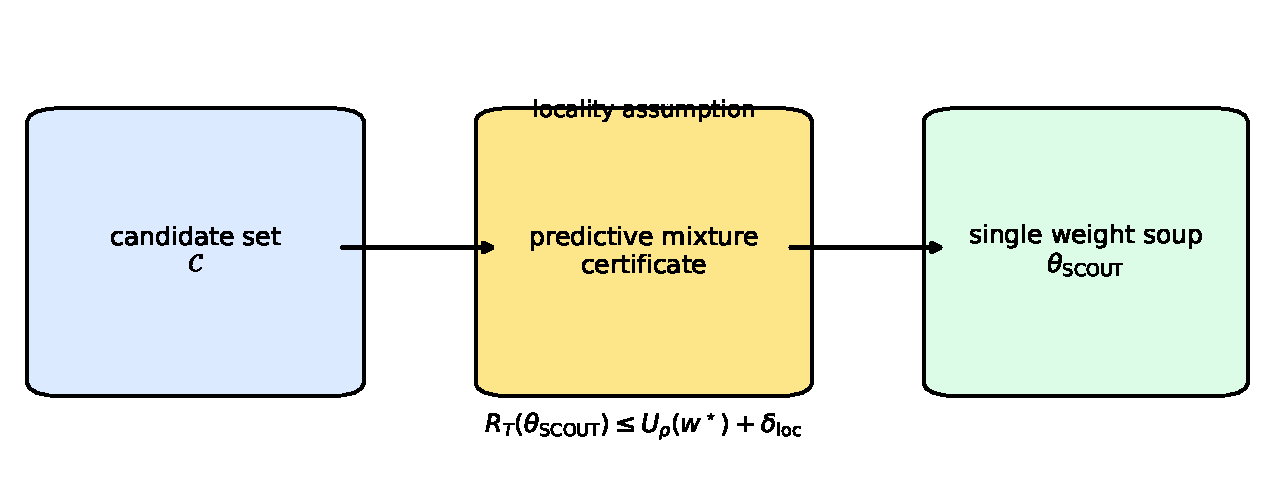
\includegraphics[width=\linewidth]{figures/soup_transfer_bridge.pdf}
    \caption{\textbf{Soup transfer bridge.} The optimization happens on predictive mixtures over the support set, but the deployed object is a single weight soup. The locality assumption is the bridge between those two objects. This is the same conceptual role that locality plays in \diwa{} and model soups, but here it is attached to a direct robust objective rather than a heuristic selector.}
    \label{fig:transfer}
\end{figure}

\subsection{Optimization guarantee}

\begin{theorem}[Projected primal--dual convergence]
\label{thm:convergence}
Suppose \(G\) is evaluated on \(\cW_M\times \cR_\rho\) with step size \(\eta>0\). Let
\[
    \bar w_T = \frac{1}{T}\sum_{t=1}^{T} w^t,
    \qquad
    \bar r_T = \frac{1}{T}\sum_{t=1}^{T} r^t.
\]
Then the iterates of Algorithm~\ref{alg:scout} satisfy
\begin{equation}
    \max_{w\in\cW_M} G(w,\bar r_T)
    -
    \min_{r\in\cR_\rho} G(\bar w_T,r)
    \le
    \frac{D_W^2 + D_R^2}{2\eta T}
    +
    \frac{\eta L^2}{2},
    \label{eq:convergence}
\end{equation}
where \(D_W\) and \(D_R\) are Euclidean diameters of \(\cW_M\) and \(\cR_\rho\), and \(L\) is a joint gradient bound for \(G\). Choosing \(\eta = \sqrt{(D_W^2+D_R^2)/(L^2 T)}\) gives a saddle residual of order \(O(T^{-1/2})\).
\end{theorem}

This is the paper's formal answer to the ``no post-hoc justification'' requirement. The method is not searching for a surrogate that might correlate with the theory. It directly solves the theory object and has a standard first-order convergence guarantee for doing so.

\subsection{Comparison to \swad{} and interval selectors}

For a contiguous interval \(I\subseteq \cC\) of length \(M\), define the corresponding uniform interval soup \(u_I\). Let
\[
    \mathfrak{I}_M
    \subseteq
    \cW_M
    \cap \{u_S:S\in\mathfrak{S}_M\}
\]
denote the feasible family of contiguous uniform interval soups of length \(M\) that satisfy the same candidate-pool restrictions.

\begin{corollary}[Certificate domination over interval families]
\label{cor:dominate}
Let \(w^\star\) be any \scout{} optimizer. Then
\begin{equation}
    \mathcal{U}_\rho(w^\star)
    \le
    \inf_{w\in \mathfrak{F}} \mathcal{U}_\rho(w)
    \label{eq:family_domination}
\end{equation}
for every feasible family \(\mathfrak{F}\subseteq \cW_M\). In particular,
\begin{equation}
    \mathcal{U}_\rho(w^\star)
    \le
    \inf_{I\in \mathfrak{I}_M} \mathcal{U}_\rho(u_I).
    \label{eq:interval_domination}
\end{equation}
Under Assumption~\ref{ass:locality}, the same domination holds for the certified target-risk upper bound in \eqref{eq:certificate}.
\end{corollary}

This is the strongest honest ``better than \swad{}'' theorem we can give without target labels. It does not claim universal empirical superiority. It says something sharper and fully defensible: once the action family and certificate are fixed, \scout{} is no worse than any contained \swad{}-style interval selector on that certificate.

\subsection{Why \dcola{} works and why \scout{} is more principled}

\begin{proposition}[Second-order redundancy penalty]
\label{prop:second_order}
Fix \(r\in\cR_\rho\) and \(w\in\cW_M\). For any perturbation \(h\in\RR^{|\cC|}\) such that \(\ones^\top h = 0\), \(w+h\in\cW_M\), and all coordinates remain positive, we have
\begin{equation}
    G(w+h,r)
    =
    G(w,r)
    +
    \inner{\nabla_w G(w,r)}{h}
    -
    \frac{1}{2}
    h^\top H(w,r) h
    +
    R_3(h),
    \label{eq:taylor}
\end{equation}
where
\begin{equation}
    H(w,r)
    =
    \sum_{i=1}^{n}
    r_i
    \frac{q_i q_i^\top}{\left(\eps_0 + q_i^\top w\right)^2},
    \qquad
    q_i = (q_{it})_{t\in\cC},
    \label{eq:hessian}
\end{equation}
is positive semidefinite, and the remainder obeys \(|R_3(h)|\le C \norm{h}_2^3\) for an explicit constant \(C\) depending on \(\eps_0\) and \(\max_{i,t} q_{it}\).
\end{proposition}

Proposition~\ref{prop:second_order} clarifies why covariance-aware soups such as \dcola{} work well empirically. The exact \scout{} objective already contains a data-adaptive redundancy penalty in its Hessian. Pairwise covariance penalties are therefore not wrong; they are low-order surrogates of the true robust coverage geometry. The difference is that \scout{} optimizes the exact object directly.

\begin{figure}[t]
    \centering
    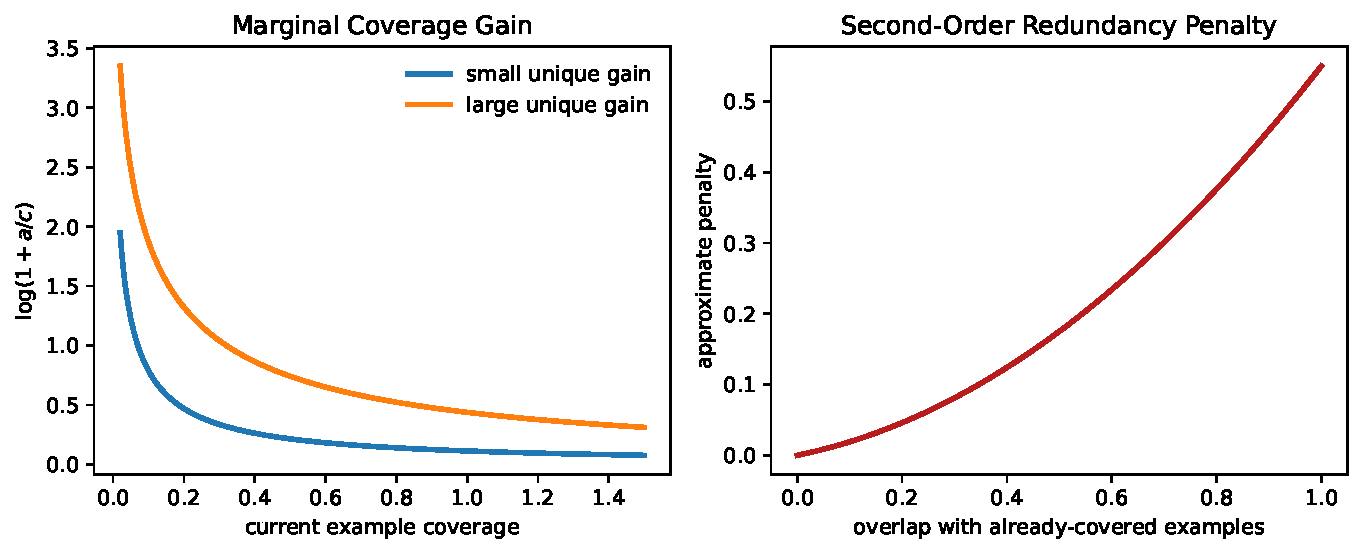
\includegraphics[width=\linewidth]{figures/diminishing_returns_vs_redundancy.pdf}
    \caption{\textbf{Diminishing returns and redundancy.} The \scout{} coverage utility rewards unique help on hard examples, but the gain decays as those examples become covered. The second-order term behaves like a redundancy penalty, which is why covariance-aware heuristics can work even though they are not direct optimizers of the exact robust objective.}
    \label{fig:diminishing}
\end{figure}

\subsection{Constructive separation from contiguous-window selectors}

\begin{theorem}[Noncontiguous complementarity separation]
\label{thm:separation}
There exists a trajectory of four feasible checkpoints ordered in time, a support set of two examples, and a soup size \(M=2\) such that:
\begin{enumerate}[leftmargin=1.4em]
    \item the \scout{} optimizer chooses weights supported on the noncontiguous pair \(\{1,4\}\),
    \item every singleton checkpoint has strictly worse robust objective value, and
    \item every contiguous interval of length \(2\) has strictly worse robust objective value.
\end{enumerate}
\end{theorem}

The proof is constructive and appears in the appendix. The point is not merely that noncontiguity can help. It is that there exist simple cases where any contiguous-window selector is structurally incapable of reaching the best robust soup.

\begin{figure}[t]
    \centering
    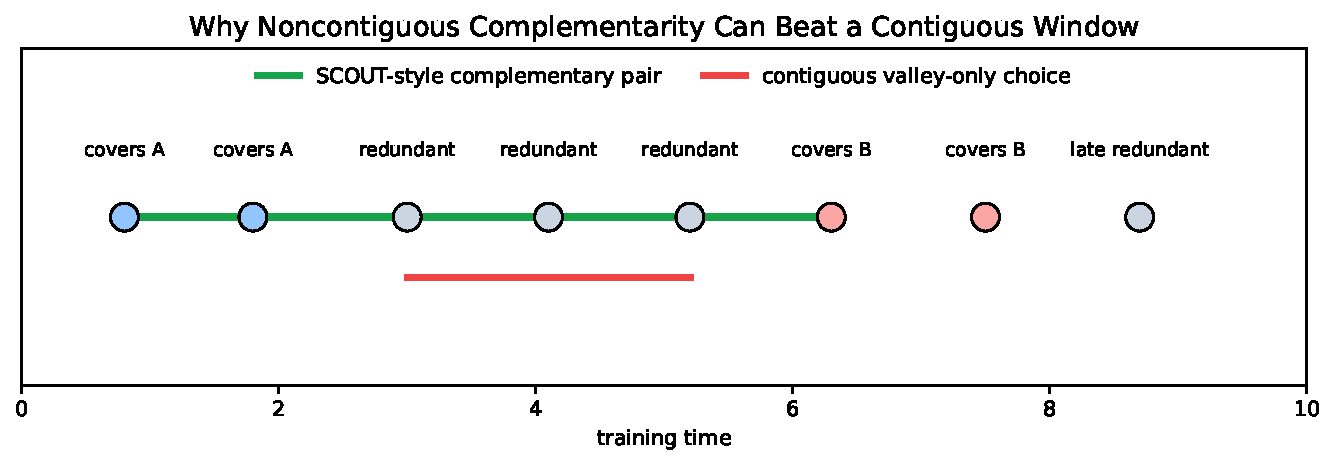
\includegraphics[width=\linewidth]{figures/noncontiguous_complementarity_toy.pdf}
    \caption{\textbf{Toy separation intuition.} If early checkpoints cover one hard subset and late checkpoints cover another, the best robust soup can be noncontiguous even when all candidate checkpoints are individually soup-safe. This is the structural regime where \scout{} can beat interval-only post-hoc selectors.}
    \label{fig:toy}
\end{figure}

\section{Experimental Protocol and Published Reference Numbers}
\label{sec:experiments}

\subsection{Protocol to be executed}

All new \scout{} experiments are intentionally left as \TBD{}. The intended protocol is:
\begin{itemize}[leftmargin=1.4em]
    \item base training under the standard DomainBed settings,
    \item dense checkpoint saving from a single run,
    \item post-hoc selection using only pooled source holdout data and no domain labels,
    \item one final test-time soup,
    \item comparison against ERM, \swad{}, \dcola{}, \cora{}, and \roar{} on the same checkpoint banks.
\end{itemize}

The first experiments that matter most are:
\begin{enumerate}[leftmargin=1.4em]
    \item replay-on-the-same-bank comparisons against \swad{} and \dcola{},
    \item ablations on \(M\), \(\rho\), \(\eps\), and \(\tau\),
    \item correlation plots between robust-support objective value and target \ood{} accuracy across dense checkpoints,
    \item decomposition studies showing when \scout{} returns extreme-point uniform soups versus interior capped-simplex soups.
\end{enumerate}

\subsection{Published reference numbers}

Table~\ref{tab:published} collects exact published numbers from prior work. These are reference points only: the protocols are not fully identical, especially for \diwa{} and \miro{}.

\begin{table}[t]
    \centering
    \small
    \caption{\textbf{Published reference numbers from prior work.} These rows are reproduced from the cited papers and are included only to define the current frontier. The protocols are not identical across rows, so this table should not be read as a new apples-to-apples comparison.}
    \label{tab:published}
    \adjustbox{width=\textwidth}{%
    \begin{tabular}{@{}llcccccc@{}}
        \toprule
        Method & Source/protocol & PACS & VLCS & OfficeHome & TerraInc & DomainNet & Avg. \\
        \midrule
        ERM & \swad{} paper, ResNet-50 & 85.5 & 77.5 & 66.5 & 46.1 & 40.9 & 63.3 \\
        \swad{} & \swad{} paper, ResNet-50 & 88.1 & 79.1 & 70.6 & 50.0 & 46.5 & 66.9 \\
        \diwa{} & \diwa{} paper, LP init, \(M=60\) & 89.0 & 78.6 & 72.8 & 51.9 & 47.7 & 68.0 \\
        \miro{} & \miro{} paper, ResNet-50 & 85.4 & 79.0 & 70.5 & 50.4 & 44.3 & 65.9 \\
        \miro{} + \swad{} & \miro{} paper, ResNet-50 & 88.4 & 79.6 & 72.4 & 52.9 & 47.0 & 68.1 \\
        \bottomrule
    \end{tabular}
    }
\end{table}

\subsection{New \scout{} results}

\paragraph{Main table.}
\TBD{}

\paragraph{Replay comparison against \swad{}, \dcola{}, \cora{}, and \roar{}.}
\TBD{}

\paragraph{Ablations on \(M\), \(\rho\), and the candidate-pool thresholds.}
\TBD{}

\paragraph{Checkpoint-bank analysis and robust-objective diagnostics.}
\TBD{}

\section{Discussion}

\paragraph{Why this is more principled than the existing post-hoc soups.}
The main advantage of \scout{} is not that it introduces one more checkpoint score. It is that the theory, the objective, and the optimizer finally line up. The action family is explicit. The uncertainty model is explicit. The certificate is explicit. The optimizer acts on that exact certificate. That is the standard a serious post-hoc DG method should meet.

\paragraph{Why this could still fail.}
\scout{} is not a free lunch. If the target shift is not well captured by bounded example reweightings of source support, the DRO assumption may be too coarse. If the barrier-filtered candidate set is too broad, soup transfer may fail. If it is too narrow, the method may collapse back into a valley selector. And if the hardest support examples are simply mislabeled or highly noisy, robust reweighting may over-focus on them. These are real risks and should be tested directly.

\paragraph{What success would look like.}
The strongest possible empirical outcome would not merely be beating \swad{} on a benchmark table. It would be a pattern:
\begin{itemize}[leftmargin=1.4em]
    \item \scout{} matches or beats \dcola{} on the same checkpoint banks,
    \item the final learned weights remain spread under the capped-simplex constraint rather than collapsing to one checkpoint,
    \item and the robust-support objective correlates with target accuracy better than flatness-only or calmness-only diagnostics.
\end{itemize}

\section{Conclusion}

This paper proposed \scout{}, a new post-hoc DG method built around a simple demand: the post-hoc selector should directly optimize the same object that appears in its target-risk certificate. \scout{} does this by combining a soup-safe candidate pool, a label-free KL-ball reweighting model over source-support examples, and a robust concave coverage objective over the convex hull of uniform subset soups. The result is a single weight soup, not an ensemble; a direct optimizer, not a window heuristic; and a theory whose main claims are about the deployed object itself. The remaining question is empirical. All new \scout{} result cells in this draft are marked \TBD{}. If the forthcoming experiments confirm that robust coverage over averageable subset soups captures what the current best checkpoint soups are actually doing, then \scout{} would provide both the cleaner theory and the stronger method that the current post-hoc DG landscape lacks.

\bibliographystyle{plainnat}
\bibliography{references}

\appendix

\section{Additional Discussion of the Objective}

For classification, \(q_{it}\) is the clipped true-class probability. The robust loss \(\mathcal{U}_\rho(w)\) is therefore a DRO version of cross-entropy on the predictive mixture induced by \(w\). The log utility \(G(w,r)\) is simply its sign-flipped form. All core theorems are about this exact deployed-object surrogate.

\section{Proofs}

\subsection{Proof of Proposition~\ref{prop:hypersimplex}}

\begin{proof}
Every vector \(u_S\) is in the capped simplex because it is nonnegative, sums to one, and each coordinate is either \(0\) or \(1/M\). Hence
\[
    \operatorname{conv}\{u_S:S\in\mathfrak{S}_M\}
    \subseteq
    \{w\in\simplex^{|\cC|-1}: 0\le w_t\le 1/M\}.
\]

For the reverse inclusion, consider
\[
    \cH_M
    \triangleq
    \left\{
        z\in [0,1]^{|\cC|} :
        \sum_{t\in\cC} z_t = M
    \right\}.
\]
This is the classical hypersimplex. Its extreme points are exactly the \(0/1\) vectors with exactly \(M\) ones. Dividing by \(M\) maps \(\cH_M\) affinely onto
\[
    \left\{
        w\in\simplex^{|\cC|-1}: 0\le w_t\le 1/M
    \right\},
\]
and maps each extreme point to a vector \(u_S\) for some \(S\in\mathfrak{S}_M\). Therefore the image of \(\cH_M\) is exactly the convex hull of the \(u_S\), which proves \eqref{eq:hypersimplex}.
\end{proof}

\subsection{Proof of Proposition~\ref{prop:submod}}

\begin{proof}
Fix \(r\in\cR_\rho\). For each example \(i\), define the modular set function
\[
    m_i(S)
    \triangleq
    \frac{1}{M}\sum_{t\in S} q_{it}.
\]
Since \(q_{it}\ge 0\), \(m_i\) is monotone modular. The scalar function
\[
    \phi_i(z) = \log(\eps_0 + z)
\]
is increasing and concave on \([0,\infty)\). Therefore the composition \(S\mapsto \phi_i(m_i(S))\) is monotone submodular. Summing with nonnegative weights \(r_i\) preserves monotone submodularity, so \(F_r\) is monotone submodular.

Now fix \(r\). The map \(w\mapsto \sum_t w_t q_{it}\) is affine, and \(z\mapsto \log(\eps_0+z)\) is concave, so each term in \(G(w,r)\) is concave in \(w\). Their nonnegative weighted sum is therefore concave on \(\cW_M\). Finally, for fixed \(w\), the map \(r\mapsto G(w,r)\) is linear because \(r\) appears only as coefficients multiplying constants
\(
    \log(\eps_0+\sum_t w_t q_{it}).
\)
Since \(\cW_M\) and \(\cR_\rho\) are compact convex sets, a saddle point exists by standard concave--convex minimax theory.
\end{proof}

\subsection{Proof of Theorem~\ref{thm:certificate}}

\begin{proof}
By Assumption~\ref{ass:reweight},
\[
    R_T^{\mathrm{mix}}(w)
    =
    \sum_{i=1}^{n} r_i^{\mathrm{T}}
    \Big[
        -\log q_w(x_i,y_i)
    \Big].
\]
Since \(r^{\mathrm{T}}\in\cR_\rho\), the definition of \(\mathcal{U}_\rho(w)\) gives
\[
    R_T^{\mathrm{mix}}(w)
    \le
    \sup_{r\in\cR_\rho}
    \sum_{i=1}^{n} r_i
    \Big[
        -\log q_w(x_i,y_i)
    \Big]
    =
    \mathcal{U}_\rho(w).
\]
Applying Assumption~\ref{ass:locality} yields
\[
    R_T(\theta_w)
    \le
    R_T^{\mathrm{mix}}(w) + \delta_{\mathrm{loc}}(w)
    \le
    \mathcal{U}_\rho(w) + \delta_{\mathrm{loc}}(w).
\]
This proves \eqref{eq:certificate}. Since \(w^\star\) minimizes \(\mathcal{U}_\rho\) over \(\cW_M\), it minimizes the certificate up to the locality residual when the latter is treated as part of the feasibility model or separately controlled by the barrier threshold.
\end{proof}

\subsection{Proof of Theorem~\ref{thm:convergence}}

\begin{proof}
The proof is the standard projected primal--dual argument for compact concave--convex saddle problems. Because \(q_{it}\in[\eps_p,1]\) and \(\eps_0>0\), the gradients in \eqref{eq:w_grad}--\eqref{eq:r_grad} are bounded on \(\cW_M\times\cR_\rho\); let \(L\) be a common bound on the joint gradient norm.

By nonexpansiveness of Euclidean projection, for any \(w\in\cW_M\),
\[
    \norm{w^{t+1}-w}^2
    \le
    \norm{w^t-w}^2
    + \eta^2 \norm{\nabla_w G(w^t,r^t)}^2
    + 2\eta \inner{\nabla_w G(w^t,r^t)}{w^t-w}.
\]
Rearranging and using concavity of \(G(\cdot,r^t)\),
\[
    G(w,r^t) - G(w^t,r^t)
    \le
    \frac{\norm{w^t-w}^2 - \norm{w^{t+1}-w}^2}{2\eta}
    +
    \frac{\eta L^2}{2}.
\]
Similarly, for any \(r\in\cR_\rho\), convexity in \(r\) gives
\[
    G(w^t,r^t) - G(w^t,r)
    \le
    \frac{\norm{r^t-r}^2 - \norm{r^{t+1}-r}^2}{2\eta}
    +
    \frac{\eta L^2}{2}.
\]
Adding the two inequalities, summing from \(t=1\) to \(T\), and telescoping yields
\[
    \sum_{t=1}^{T}
    \Big(
        G(w,r^t) - G(w^t,r)
    \Big)
    \le
    \frac{D_W^2 + D_R^2}{2\eta}
    +
    \eta L^2 T,
\]
where \(D_W\) and \(D_R\) are diameters of \(\cW_M\) and \(\cR_\rho\). Dividing by \(T\) and applying Jensen's inequality to the concave map \(w\mapsto G(w,\bar r_T)\) and linearity in \(r\) gives
\[
    \max_{w\in\cW_M} G(w,\bar r_T)
    -
    \min_{r\in\cR_\rho} G(\bar w_T,r)
    \le
    \frac{D_W^2 + D_R^2}{2\eta T}
    +
    \frac{\eta L^2}{2}.
\]
Choosing \(\eta\) to balance the terms yields the \(O(T^{-1/2})\) rate.
\end{proof}

\subsection{Proof of Corollary~\ref{cor:dominate}}

\begin{proof}
By definition, \(w^\star\) minimizes \(\mathcal{U}_\rho(w)\) over the whole feasible set \(\cW_M\). Therefore for any \(\mathfrak{F}\subseteq\cW_M\),
\[
    \mathcal{U}_\rho(w^\star)
    \le
    \inf_{w\in\mathfrak{F}} \mathcal{U}_\rho(w).
\]
Taking \(\mathfrak{F}=\mathfrak{I}_M\) gives \eqref{eq:interval_domination}. Under Assumption~\ref{ass:locality}, adding the same locality residual model to both sides preserves domination of the certified upper bound.
\end{proof}

\subsection{Proof of Proposition~\ref{prop:second_order}}

\begin{proof}
Define
\[
    c_i(w) \triangleq \eps_0 + q_i^\top w.
\]
Then
\[
    G(w+h,r)
    =
    \sum_{i=1}^{n} r_i \log(c_i(w) + q_i^\top h).
\]
Applying the scalar Taylor expansion
\[
    \log(c+z)
    =
    \log c + \frac{z}{c} - \frac{z^2}{2c^2} + \frac{z^3}{3\xi^3},
\]
for some \(\xi\) between \(c\) and \(c+z\), to each term gives
\[
    G(w+h,r)
    =
    G(w,r)
    +
    \sum_{i=1}^{n} r_i \frac{q_i^\top h}{c_i(w)}
    -
    \frac{1}{2}
    \sum_{i=1}^{n} r_i \frac{(q_i^\top h)^2}{c_i(w)^2}
    +
    R_3(h).
\]
The first-order term is \(\inner{\nabla_w G(w,r)}{h}\). The quadratic term can be written as
\[
    \frac{1}{2}
    h^\top
    \left(
        \sum_{i=1}^{n}
        r_i \frac{q_i q_i^\top}{c_i(w)^2}
    \right)
    h
    =
    \frac{1}{2} h^\top H(w,r) h.
\]
Each matrix \(q_i q_i^\top\) is positive semidefinite and the coefficients \(r_i/c_i(w)^2\) are nonnegative, so \(H(w,r)\) is positive semidefinite.

For the remainder, note that \(c_i(w)\ge \eps_0\) and \(q_i^\top h\) is bounded by \(\norm{q_i}_\infty \norm{h}_1\). Hence the scalar third-order remainder is bounded by a constant times \(|q_i^\top h|^3/\eps_0^3\). Summing over \(i\) yields \(|R_3(h)|\le C\norm{h}_2^3\) for an explicit \(C\) depending only on \(\eps_0\), \(r\), and the \(q_i\).
\end{proof}

\subsection{Proof of Theorem~\ref{thm:separation}}

\begin{proof}
Take four checkpoints in temporal order \(1,2,3,4\), soup size \(M=2\), and two support examples \(A,B\). Let the clipped true-class probabilities be
\[
    q_A = (0.99, 0.60, 0.40, 0.20),
    \qquad
    q_B = (0.20, 0.40, 0.60, 0.99).
\]
Assume every checkpoint is feasible, so every pair satisfying the cardinality rule lies in the action space.

For the noncontiguous pair \(\{1,4\}\), the uniform soup gives
\[
    \frac{q_A(1)+q_A(4)}{2}
    =
    \frac{0.99+0.20}{2}
    = 0.595,
    \qquad
    \frac{q_B(1)+q_B(4)}{2}
    =
    \frac{0.20+0.99}{2}
    = 0.595.
\]
Therefore its robust loss under any adversary on \(\{A,B\}\) is
\[
    -\log 0.595.
\]

Now check every contiguous interval of length two:
\[
    \{1,2\}:
    \Big(
        \frac{0.99+0.60}{2},
        \frac{0.20+0.40}{2}
    \Big)
    =
    (0.795,0.30),
\]
\[
    \{2,3\}:
    \Big(
        \frac{0.60+0.40}{2},
        \frac{0.40+0.60}{2}
    \Big)
    =
    (0.50,0.50),
\]
\[
    \{3,4\}:
    \Big(
        \frac{0.40+0.20}{2},
        \frac{0.60+0.99}{2}
    \Big)
    =
    (0.30,0.795).
\]
Under worst-case reweighting of the two examples, their robust losses are respectively
\[
    -\log 0.30,\qquad -\log 0.50,\qquad -\log 0.30,
\]
all strictly larger than \(-\log 0.595\). Every singleton has worst-case probability at most \(0.40\) on one of the two examples and therefore robust loss at least \(-\log 0.40\), also strictly worse than \(-\log 0.595\). Hence the noncontiguous pair \(\{1,4\}\) strictly dominates every singleton and every contiguous interval.
\end{proof}

\section{Planned Experimental Tables}

\paragraph{Main apples-to-apples benchmark table.}
\TBD{}

\paragraph{Replay-bank comparison table.}
\TBD{}

\paragraph{Ablation table for \(M\), \(\rho\), \(\eps\), and \(\tau\).}
\TBD{}

\paragraph{Calibration of the support-reweighting adversary.}
\TBD{}

\section{Additional Figures}

\begin{figure}[H]
    \centering
    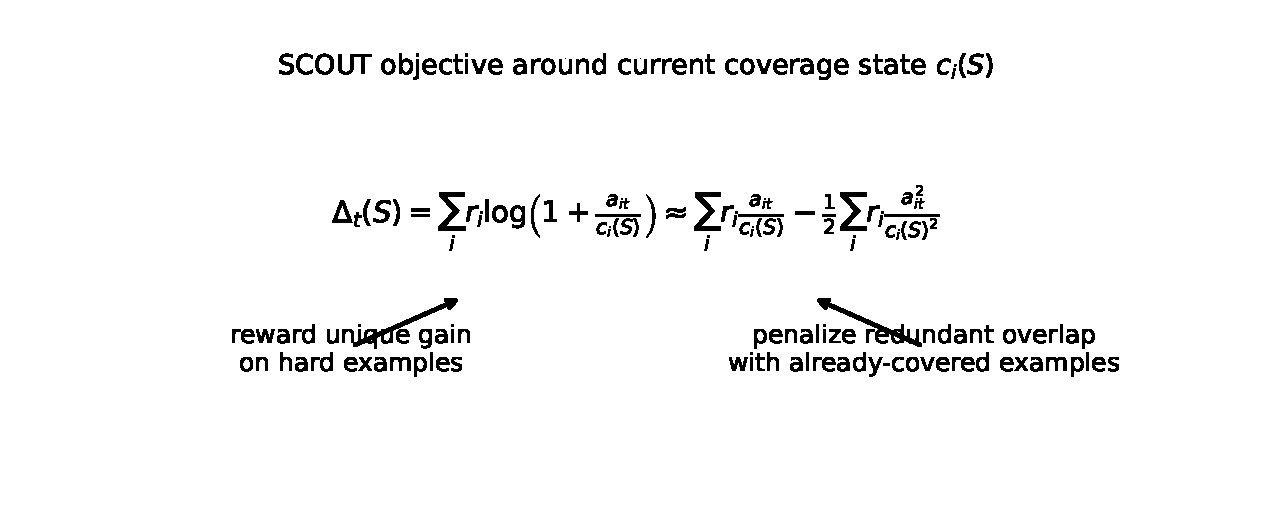
\includegraphics[width=\linewidth]{figures/surrogate_link_to_dcola.pdf}
    \caption{\textbf{How \dcola{}-style surrogates arise.} The exact \scout{} marginal-gain expression reduces to a first-order reward for unique help on hard examples and a second-order redundancy penalty. This is why covariance-aware checkpoint soups can work empirically even when they do not directly optimize the robust target certificate.}
    \label{fig:surrogate}
\end{figure}

\end{document}
